\documentclass[
	a4paper,
	oneside,
	BCOR = 10mm,
	DIV = 12,
	12pt,
	headings = normal,
]{scrartcl}

%%% Length calculations
\usepackage{calc}
%%%

%%% Support for color
\usepackage{xcolor}
\definecolor{lightblue}{HTML}{03A9F4}
\definecolor{red}{HTML}{F44336}
%%%

%%% Including graphics
\usepackage{graphicx}
%%%

%%% Font selection
\usepackage{fontspec}

\setromanfont{STIX Two Text}[
	SmallCapsFeatures = {LetterSpace = 8},
]

\setsansfont{IBM Plex Sans}[
	Scale = MatchUppercase,
]

\setmonofont{IBM Plex Mono}[
	Scale = MatchUppercase,
]
%%%

%%% Math typesetting
\usepackage{amsmath}

\usepackage{unicode-math}
\setmathfont{STIX Two Math}

\usepackage{IEEEtrantools}
%%%

%%% List settings
\usepackage{enumitem}
\setlist[enumerate]{
	label*      = {\arabic*.},
	left        = \parindent,
	topsep      = 0\baselineskip,
	parsep      = 0\baselineskip,
	noitemsep, % override itemsep
}
% List settings for levels 2–4
\setlist[enumerate, 2, 3, 4]{
	label*      = {\arabic*.},
	left        = 0em,
	topsep      = 0\baselineskip,
	parsep      = 0\baselineskip,
	noitemsep, % override itemsep
}

\setlist[itemize]{
	label*      = {—},
	left        = \parindent,
	topsep      = 0\baselineskip,
	parsep      = 0\baselineskip,
	itemsep     = 1\baselineskip,
	noitemsep, % override itemsep
}

\setlist[description]{
	font        = {\rmfamily\upshape\bfseries},
	topsep      = 1\baselineskip,
	parsep      = 0\baselineskip,
	itemsep     = 0\baselineskip,
}

%%%

%%% Structural elements typesetting
\setkomafont{pagenumber}{\rmfamily\upshape}
\setkomafont{disposition}{\rmfamily\bfseries}

% Sectioning
\RedeclareSectionCommand[
	beforeskip = -1\baselineskip,
	afterskip  = 1\baselineskip,
	font       = {\normalsize\bfseries\scshape},
]{section}

\RedeclareSectionCommand[
	beforeskip = -1\baselineskip,
	afterskip  = 1\baselineskip,
	font       = {\normalsize\bfseries\itshape},
]{subsection}

\RedeclareSectionCommand[
	beforeskip = -1\baselineskip,
	afterskip  = 1\baselineskip,
	font       = {\normalsize\bfseries},
]{subsubsection}

\RedeclareSectionCommand[
	beforeskip = -1\baselineskip,
	afterskip  = -0.5em,
	font       = {\normalsize\mdseries\scshape\addfontfeatures{Letters = {UppercaseSmallCaps}}},
]{paragraph}
%%%

%%% Typographic enhancements
\usepackage{microtype}
%%%

%%% Language-specific settings
\usepackage{polyglossia}
\setmainlanguage{ukrainian}
\setotherlanguages{english}
%%%

%%% Captions
\usepackage{caption}
\usepackage{subcaption}

%\DeclareCaptionLabelFormat{closing}{#2)}
%\captionsetup[subtable]{labelformat = closing}

%\captionsetup[subfigure]{labelformat = closing}

\captionsetup[table]{
	aboveskip = 0\baselineskip,
	belowskip = 0\baselineskip,
}

\captionsetup[figure]{
	aboveskip = 1\baselineskip,
	belowskip = 0\baselineskip,
}

\captionsetup[subfigure]{
	labelformat = simple,
	labelformat = brace,
}
%%%

%%% Hyphenated ragged typesetting
\usepackage{ragged2e}
%%%

%%% Table typesetting
\usepackage{booktabs}
\usepackage{longtable}

\usepackage{multirow}

\usepackage{array}
\newcolumntype{v}[1]{>{\RaggedRight\arraybackslash\hspace{0pt}}p{#1}}
\newcolumntype{b}[1]{>{\Centering\arraybackslash\hspace{0pt}}p{#1}}
\newcolumntype{n}[1]{>{\RaggedLeft\arraybackslash\hspace{0pt}}p{#1}}
%%%

%%% Drawing
\usepackage{tikz}
\usepackage{tikzscale}
\usetikzlibrary{positioning}
\usetikzlibrary{arrows.meta} % Stealth arrow tips
%%%

%%% SI units typesetting
\usepackage{siunitx}
\sisetup{
	output-decimal-marker = {,},
	exponent-product      = {\cdot},
	inter-unit-product    = \ensuremath{{} \cdot {}},
	per-mode              = symbol,
}
%%%

% Code Highlighting
\usepackage{minted}
\setmintedinline{
	style = bw,
	breaklines,
}

\newminted[bashterm]{bash}{%
	autogobble,%
	style=bw,%
}

\newmintinline{bash}{%
}

%%% Framing code listings
\usepackage{tcolorbox}
\tcbuselibrary{breakable}
\tcbuselibrary{minted}
\tcbuselibrary{skins}

% Text file listing
\newtcblisting[
	auto counter,
	list inside, 
	number within = section,
]{listingplaintext}[3][]{%
	minted language = text,
	minted style    = bw,
	minted options  = {
		autogobble,
		linenos,
		tabsize = 4,
		breaklines,
		breakanywhere,
		fontsize = \footnotesize,
	},
	empty,
	sharp corners,
	coltitle = black,
	borderline horizontal = {1pt}{0pt}{black},
	titlerule = {0.5pt},
	titlerule style = {
		black,
	},
	toptitle = 0.3em,
	bottomtitle = 0.3em,
	before skip      = \intextsep,
	after  skip      = \intextsep,
	title            = {Лістинг \thetcbcounter: #2},
	list entry       = {\protect\numberline{\thetcbcounter}#2},
	left = 0em,
	right = 0em,
	%
	listing only,
	breakable,
	%
	label = {#3},%
}

\newtcblisting[
	use counter from = listingplaintext,
	list inside, 
	number within = section,
]{listingpython}[3][]{%
	minted language = python,
	minted style    = bw,
	minted options  = {
		autogobble,
		linenos,
		tabsize = 4,
		breaklines,
		breakanywhere,
		fontsize = \footnotesize,
	},
	empty,
	sharp corners,
	coltitle = black,
	borderline horizontal = {1pt}{0pt}{black},
	titlerule = {0.5pt},
	titlerule style = {
		black,
	},
	toptitle = 0.3em,
	bottomtitle = 0.3em,
	before skip      = \intextsep,
	after  skip      = \intextsep,
	title            = {Лістинг \thetcbcounter: #2},
	list entry       = {\protect\numberline{\thetcbcounter}#2},
	left = 0em,
	right = 0em,
	%
	listing only,
	breakable,
	%
	label = {#3},
	%
	#1%
}

\newtcbinputlisting[
	use counter from = listingplaintext,
	list inside,
	number within = section
]{\inputpython}[4][]{%
	minted language = python,
	minted style    = bw,
	minted options  = {
		autogobble,
		linenos,
		tabsize = 4,
		breaklines,
		breakanywhere,
		fontsize = \footnotesize,
	},
	empty,
	sharp corners,
	coltitle = black,
	borderline horizontal = {1pt}{0pt}{black},
	titlerule = {0.5pt},
	titlerule style = {
		black,
	},
	toptitle = 0.3em,
	bottomtitle = 0.3em,
	before skip      = \intextsep,
	after  skip      = \intextsep,
	title            = {Лістинг \thetcbcounter: #3},
	list entry       = {\protect\numberline{\thetcbcounter}#3},
	left = 0em,
	right = 0em,
	%
	listing file={#2},
	listing only,
	breakable,
	%
	label = {#4}
}

% Linux command-line listing
\newtcblisting{linuxterm}%
{%
	% Syntax highlighing options
	listing only,%
	minted language = bash,%
	minted options={%
		autogobble,%
		linenos%
	},%
	% Presentation options
	empty,%
	%% Margins
	sharp corners,%
	toptitle = 0.0em,%
	bottomtitle = 0.0em,%
	left = 0em,%
	right = 0em,%
	before skip = \intextsep,%
	after skip = \intextsep,%
}

\newtcblisting{linuxtermout}%
{%
	% Syntax highlighing options
	listing only,%
	minted language = text,%
	minted options={%
		autogobble,%
		linenos%
	},%
	% Presentation options
	empty,%
	%% Margins
	sharp corners,%
	toptitle = 0.0em,%
	bottomtitle = 0.0em,%
	left = 0em,%
	right = 0em,%
	before skip = \intextsep,%
	after skip = \intextsep,%
}

% Dockerfile listings
\newtcblisting[
	use counter from = listingplaintext,
	list inside, 
	number within = section,
]{listingdocker}[3][]{%
	minted language = dockerfile,
	minted style    = bw,
	minted options  = {
		autogobble,%
		linenos,
		tabsize = 4,
		breaklines,
		breakanywhere,
		fontsize = \footnotesize,
	},
	empty,
	sharp corners,
	coltitle = black,
	borderline horizontal = {1pt}{0pt}{black},
	titlerule = {0.5pt},
	titlerule style = {
		black,
	},
	toptitle = 0.3em,
	bottomtitle = 0.3em,
	before skip      = \intextsep,
	after  skip      = \intextsep,
	title            = {Лістинг \thetcbcounter: #2},
	list entry       = {\protect\numberline{\thetcbcounter}#2},
	left = 0em,
	right = 0em,
	%
	listing only,
	breakable,
	%
	label = {#3},%
}

% Docker Compose listings
\newtcblisting[
	use counter from = listingplaintext,
	list inside, 
	number within = section,
]{listingdockercompose}[3][]{%
	minted language = yaml,
	minted style    = bw,
	minted options  = {
		autogobble,%
		linenos,
		tabsize = 4,
		breaklines,
		breakanywhere,
		fontsize = \footnotesize,
	},
	empty,
	sharp corners,
	coltitle = black,
	borderline horizontal = {1pt}{0pt}{black},
	titlerule = {0.5pt},
	titlerule style = {
		black,
	},
	toptitle = 0.3em,
	bottomtitle = 0.3em,
	before skip      = \intextsep,
	after  skip      = \intextsep,
	title            = {Лістинг \thetcbcounter: #2},
	list entry       = {\protect\numberline{\thetcbcounter}#2},
	left = 0em,
	right = 0em,
	%
	listing only,
	breakable,
	%
	label = {#3},%
}

% Customize minted line numbers
\renewcommand{\theFancyVerbLine}{\ttfamily\scriptsize\arabic{FancyVerbLine}}

%%%

%%% Links and hyperreferences
\usepackage{hyperref}
\hypersetup{
	bookmarksnumbered = true,
	colorlinks      = false,
	linkbordercolor = red,
	urlbordercolor  = lightblue,
	pdfborderstyle  = {/S/U/W 1.5},
}
%%%

%%% Length adjustment

% Set baselineskip, default is 14.5 pt
\linespread{1.068966} % ~15.5 pt
\setlength{\emergencystretch}{1em}
\setlength{\parindent}{1.5em}
\newlength{\gridunitwidth}
\setlength{\gridunitwidth}{\textwidth / 12}
%%%

%%% Custom commands
\newcommand{\allcaps}[1]{%
	{%
		\addfontfeatures{%
			Letters = UppercaseSmallCaps,
			LetterSpace = 8,%
			Kerning = Off%
		}%
		#1%
	}%
}
\newcommand{\filename}[1]{\texttt{#1}}
\newcommand{\progname}[1]{\texttt{#1}}
\newcommand{\commandname}[1]{\texttt{#1}}
\newcommand{\modulename}[1]{\texttt{#1}}
\newcommand{\transeng}[1]{{англ.}~\textit{\textenglish{#1}}}
%%%

%%% Custom math commands
\newcommand{\longvar}[1]{\mathit{#1}}
%%%

\begin{document}

\begin{titlepage}
		\begin{center}
			Міністерство освіти і~науки України\\
			Національний авіаційний університет\\
			Навчально-науковий інститут комп'ютерних інформаційних технологій\\
			Кафедра комп'ютеризованих систем управління

			\vspace{\fill}
				Домашнє завдання\\
				з~дисципліни «Системне програмне забезпечення»\\
				на~тему «Платформа контейнеризації~\textenglish{Docker}»\\

			\vspace{\fill}

			\begin{flushright}
				Виконав:\\
				студент \allcaps{ННІКІТ}\\
				групи \allcaps{СП}-325\\
				Клокун В.\,Д.\\
				Перевірив:\\
				Глазок О.\,М.
			\end{flushright}

			Київ 2019
		\end{center}
	\end{titlepage}

	\tableofcontents
	\clearpage

	\section{Завдання}
		Описати платформу~\textenglish{Docker} і~основні способи її~використання.

	\section{Що~таке платформа~\textenglish{Docker}}
		\subsection{Системні засоби, які використовує платформа~\textenglish{Docker}}
			Найважливіша функціональність платформи~\textenglish{Docker} побудована на~основі засобів операційних систем, розроблених задовго до~початку розробки платформи~\textenglish{Docker}. Інновація цієї платформи в~тому, наскільки зручною вона робить використання цих засобів. Тому, щоб розібратись, що~таке платформа~\textenglish{Docker}, спочатку розглянемо системні засоби, які зумовили її~створення, на~основі яких вона побудована і~які вона використовує.

			\subsubsection{Простір ядра і~користувача}
				Щоб захистити пам'ять і~апаратне забезпечення від зловмисного використання або помилкової поведінки, сучасні операційні системи розділяють віртуальну пам'ять на~два шари: простір ядра і~простір користувача. \emph{Простір ядра}~— це~область віртуальної пам'яті, в~якій ядро операційної системи зберігається, виконується і~надає свої сервіси.

				Для правильної роботи ядру операційної системи необхідно багато функцій, що~працюють на~низькому рівні або виконують чутливі операції: прямий доступ до~апаратного забезпечення, зберігання, зчитування і~запис конфіденційних даних, виконання операцій, які при неправильному використанні можуть вивести систему з~ладу. Ці~функції є~потенційно небезпечними, бо~при неправильному використанні можуть вивести систему з~ладу або порушити її~безпеку. Крім того, більшість з~них не~потрібні користувачам напряму. Отже, в~просторі ядра зберігається виключно ядро операційної системи і~необхідні йому дані.

				Щоб підвищити рівень стабільності і~безпеки операційної системи, існує другий шар — \emph{простір користувача}, тобто місце, де~зберігається і~виконується прикладний код і~необхідні йому дані (користувацьких програм тощо). Інакше кажучи, у~просторі користувача зберігається все, що~не~є~ядром операційної системи: код бібліотек і~прикладних виконуваних файлів, процеси користувачів тощо.
				
				Порівняно із~системним кодом, код, що~виконується у~користувацькому просторі, має менший доступ до~ресурсів системи і~менше прав з~метою безпеки. Щоб отримати доступ до~ресурсів ядра операційної системи, код з~простору користувача викликає спеціальні функції~— \emph{системні виклики}.
			
			\subsubsection{Віртуалізація на~рівні операційної системи}
				Такий підхід дозволяє використовувати технологію віртуалізації на~рівні операційної системи~— таку технологію віртуалізації, при якій ядро операційної системи надає можливість створювати декілька ізольованих інстанцій користувацького простору. При віртуалізації на~рівні операційної системи ядро операційної системи залишається одним і~тим же, змінюється лише простір користувача: системні бібліотеки, програми, файлова система, середовище виконання~(\transeng{runtime environment}) тощо.

		\subsection{Основні поняття платформи~\textenglish{Docker}}
			\label{ssec:docker-main-concepts}
			\textenglish{Docker}~— це~програмна платформа для віртуалізації на~рівні операційної системи. Вона дозволяє розробляти, розгортати і~запускати прикладні програми за~допомогою контейнерів. Використання контейнерів для розгортання прикладних програм називається \emph{контейнеризацією}. Контейнеризація стала популярною технологією, бо~контейнери:
			\begin{enumerate}
				\item Гнучкі. Навіть найскладніші прикладні програми можна контейнеризувати.
				\item Легкі. Контейнери використовують ядро основної операційної системи.
				\item Легкозамінні. Можна розгортати оновлення «на~льоту», під час роботи існуючого контейнера.
				\item Портативні. Можна побудувати контейнер на~одному комп'ютері, завантажити його на~віддалений сервер і~запустити будь-де.
				\item Масштабовані. Можна збільшувати і~автоматично розподіляти кон\-тей\-не\-ри-ре\-плі\-ки.
				\item Нагромаджувані~(\transeng{stackable})~— можна нагромаджувати сервіси вертикально і~«на~льоту».
			\end{enumerate}

			\paragraph{Образи і~контейнери}
				У~контексті платформи~\textenglish{Docker}, \emph{образом} називається виконуваний пакет, який містить усі засоби, необхідні для запуску прикладної програми: її~код, середовище виконання, бібліотеки, змінні середовища~(\transeng{environment variables}) і~конфігураційні файли. Коли образ запускають на~виконання, з'являється \emph{контейнер}~— конкретний запущений примірник певного образу.

			\paragraph{Контейнери і~віртуальні машини}
				На~відміну від віртуальних машин, які запускають повноцінну гостьову операційну систему, щоб виконувати у~ній потрібні програми, контейнери запускаються безпосередньо на~операційній системі~— хазяїні~(\transeng{host operating system}), використовують її~ядро і~ресурси напряму. Тим не~менш, ядро операційної системи повністю ізолює контейнери одне від одного і~операційної системи~— хазяїна, якщо не~вказано інакше.

			\subsection{Призначення платформи~\textenglish{Docker}}
				Багатьом прикладним програмам для роботи необхідні зовнішні бібліотеки або інші засоби на~кшталт баз даних і~черг задач. Під час розробки прикладних програм, вони часто тестуються на~конкретних версіях цих зовнішніх бібліотек і~засобів, тобто їх~працездатність гарантується лише для певних версій. Однак, зазвичай на~різних обчислювальних машинах встановлені різні операційні системи, різні версії необхідних бібліотек і~засобів, або ці~засоби взагалі відсутні. Часто це~означає, що~розроблена програма не~зможе запуститись і~правильно працювати на~таких обчислювальних машинах. Ця~проблема називається \emph{проблемою управління конфігураціями}.

				Щоб вирішити цю~проблему і~уникнути необхідності вручну переконуватись, що~на~усіх машинах, де~повинна виконуватись програма, встановлені потрібні засоби правильної версії, використовують платформу~\textenglish{Docker}. Як~було сказано у~розділі~\ref{ssec:docker-main-concepts}, вона дозволяє розробляти, розгортати і~запускати прикладні програми за~допомогою контейнерів. Контейнери створюються за~допомогою образів~— виконуваних пакетів, в~яких встановлені власні бібліотеки, налаштовані середовища виконання та~інші необхідні засоби. Ці~пакети незмінні, тобто якщо запустити на~різних машинах різні контейнери, створені з~однакового образу, всередині цих контейнерів буде однакове середовище.
				
				Розробники використовують цю~властивість, щоб з~впевненістю запускати програму на~різних обчислювальних машинах. Для цього програми розроблюють так, щоб вони могли запускатись у~контейнерах: коригують архітектуру, розбиваючи її~на~модулі, створюють образ, всередині якого має працювати програма, і~коли потрібно запустити програму на~іншій машині, її~запускають за~допомогою створеного образу. Таким чином, якщо програма протестована і~налагоджена для роботи всередині описаного образу, можна впевнено стверджувати, що~вона запрацює у~будь-якому контейнері, створеному на~основі описаного образу.

				У~платформи~\textenglish{Docker} є~багато призначень, крім управління конфігураціями: поєднання контейнерів у~багатоконтейнерні сервіси, балансування навантаження, реплікація і~оркестрація (автоматичне розгортання) тощо, але всі вони базуються на~основній ідеї контейнера, створеної для управління конфігурацією одного примірника.

			\subsection{Компоненти платформи~\textenglish{Docker}}
				Платформа~\textenglish{Docker} є~«програмою як~сервісом»~(\transeng{soft\-ware-as-a-ser\-vice, \allcaps{SAAS}}), яка складається з~декількох компонентів, що~взаємодіють між собою. Такими компонентами є:
				\begin{enumerate}
					\item Прикладні програми, до~яких входять:
						\begin{enumerate}
							\item Демон~\progname{dockerd}~— постійний процес, який працює на~фоні і~керує \textenglish{Docker}-контейнерами і~об'єктами. Цей демон управляється запитами, відправленими за~допомогою~\textenglish{Docker Engine \allcaps{API}}.
							\item Програма~\progname{docker}~— прикладна клієнтська програма, яка надає командний інтерфейс для взаємодії з~демоном платформи~\textenglish{Docker}.
						\end{enumerate}
					\item Об'єкти~— різні сутності, на~основі яких складаються різні модулі прикладних програм на~платформі~\textenglish{Docker}. Такими сутностями є:
						\begin{enumerate}
							\item Контейнер~— стандартизоване ізольоване середовище, яке виконує прикладну програму або її~окремий компонент. Контейнери управляються за~допомогою командного інтерфейсу або~\textenglish{Docker \allcaps{API}}.
							\item Образ~— пакет, який містить середовище з~усім необхідним для запуску контейнера і~за~допомогою якого вони будуються. Образи використовують, щоб зберігати і~доставляти прикладні програми користувачам або іншим кінцевим точкам.
							\item Сервіс~— набір контейнерів, які можна масштабувати і~виконувати під управлінням декількох різних демонів~\textenglish{Docker}. Результат такого масштабування називають \emph{роєм}~(\transeng{swarm}).
						\end{enumerate}
					\item Регістри~— репозиторії, в~яких зберігаються \textenglish{Docker}-образи. Клієнти підключаються до~регістрів, щоб завантажити («витягнути», \transeng{pull}) образи на~свої машини або помістити (\transeng{push}) їх~у~регістр.
				\end{enumerate}
				Також платформа~\textenglish{Docker} надає утиліти, які спрощують її~використання або розширити її~функціональність, а~саме:
				\begin{enumerate}
					\item \textenglish{Docker Compose}~— утиліта для визначення, запуску і~управління прикладними програмами, побудованими на~декількох контейнерах. Сервіси, з~яких складається прикладна програма, визначаються у~спеціальних файлах формату~\textenglish{\allcaps{YAML}} під назвою~\filename{\textenglish{docker-compose.yml}}.
					\item \textenglish{Docker Swarm}~— утиліта, за~допомогою якої \textenglish{Docker}-контейнери об'єднують і~організовують у~кластери.
				\end{enumerate}
				Як~видно, платформа~\textenglish{Docker} надає повнофункціональний набір для розробки і~розгортання прикладних програм різної складності у~різних ситуаціях.

		\section{Практичне використання платформи~\textenglish{Docker}}
			\subsection{Установка платформи~\textenglish{Docker}}
				Засоби платформи~\textenglish{Docker} розповсюджується у~декількох варіантах: \textenglish{Docker Community Edition~(\allcaps{CE})} і~\textenglish{Docker Enterprise Edition~(\allcaps{EE})}. Компанія~\textenglish{Docker, Inc.} позиціонує варіант~\textenglish{Community Edition} як~ідеальний для розробників і~невеликих команд та~експериментів з~технологією контейнеризації, а~\textenglish{Enterprise Edition} як~ідеальний для компаній і~широкомасштабних рішень. Тим не~менш, інструменти~\textenglish{Docker Community Edition} є~повнофункціональними і~підходять для використання навіть для корпоративних клієнтів, тому використаємо саме цей варіант, щоб показати можливості платформи.

				На~момент виконання даного завдання продукт~\textenglish{Docker Community Edition} має дві редакції: \textenglish{Desktop} і~\textenglish{Server}. Редакція~\textenglish{Desktop} призначена для запуску на~персональних комп'ютерах, а~редакція~\textenglish{Server}~— на~серверних. Ці~версії доступні для багатьох важливих платформ~(табл.~\ref{tab:docker-compat}).

				\begin{table}[!htbp]
					\centering
					\caption{Апаратно-програмні платформи, що~підтримуються продуктом~\textenglish{Docker Community Edition} редакцій \textenglish{Desktop} і~\textenglish{Server}}
					\label{tab:docker-compat}
					\begin{tabular}{
							v{2.25\gridunitwidth - 2\tabcolsep}
							n{1.75\gridunitwidth - 2\tabcolsep}
							n{2\gridunitwidth - 2\tabcolsep}
							n{2\gridunitwidth - 2\tabcolsep}
							n{2\gridunitwidth - 2\tabcolsep}
							n{2\gridunitwidth - 2\tabcolsep}
					}
						\toprule
							Платформа & \textenglish{x86\_64~/ amd64} & \textenglish{\allcaps{ARM}} & \textenglish{ARM64 / AARCH64} & \textenglish{\allcaps{IBM} Power} & \textenglish{\allcaps{IBM}~Z}\\
						\midrule
							\multicolumn{6}{c}{\textenglish{Desktop}} \\
							\cmidrule(lr){1-6}
							Windows 10 & + &   &   &   &  \\
							macOS      & + &   &   &   &  \\
							\cmidrule(lr){1-6}
							\multicolumn{6}{c}{\textenglish{Server}} \\
							\cmidrule(lr){1-6}
							CentOS     & + &   &   &   &  \\
							Debian     & + & + & + &   &  \\
							Fedora     & + &   &   &   &  \\
							Ubuntu     & + & + & + & + & +\\
						\bottomrule
					\end{tabular}
				\end{table}

				Щоб встановити~\textenglish{Docker} на~підтримуваній платформі, треба перейти за~посиланням, де~описана інформація про установку~(\url{https://docs.docker.com/install/}), знайти потрібну платформу і~слідувати наведеним вказівкам.

				Після того, як~продукт~\textenglish{Docker} буде встановлений, варто перевірити його працездатність. Для цього виконаємо команду (можливо, знадобиться запустити команду від імені суперкористувача за~допомогою команди~\commandname{sudo}):
				\begin{linuxterm}
					docker --version
				\end{linuxterm}

				Якщо \textenglish{Docker} встановлений правильно, результат виконання команди виглядатиме приблизно так:
				\begin{linuxtermout}
					Docker version 17.12.0-ce, build c97c6d6
				\end{linuxtermout}

			\subsection{Контейнери}
				Контейнери~— це~найменша структурна одиниця платформи~\textenglish{Docker}. Усі інші структурні одиниці будуються на~основі контейнерів. Розглянемо основні задачі, які виникають під час роботи з~ними.

				\subsubsection{Створення \textenglish{Docker}-образів}
					Як~було сказано у~розділі~\ref{ssec:docker-main-concepts}, контейнери є~конкретними примірниками образів, тобто щоб запустити контейнер, треба спочатку побудувати образ. Щоб створити~\textenglish{Docker}-образ, використовують спеціальні файли, які називаються~«\textenglish{Dockerfile}». Ці~файли містять інструкції для створення образів.
					
					Розглядатимемо ці~файли на~прикладі прикладної програми~— веб-додатку, який вітатиме користувача та~виводитиме лічильник відвідувань. Веб-додаток напишемо на~мові програмування~\textenglish{Python}, використовуючи базу даних~\textenglish{Redis}. Веб-додаток складатиметься з~двох файлів: \filename{\textenglish{requirements.txt}}~(лістинг~\ref{lst:requirements-txt}) і~\filename{\textenglish{app.py}}~(лістинг~\ref{lst:app-py}).

					\begin{listingplaintext}%
					{Файл~\filename{\textenglish{requirements.txt}}, який описує модулі, необхідні для роботи веб-додатку}%
					{lst:requirements-txt}
						Flask
						Redis
					\end{listingplaintext}

					\begin{listingpython}{Файл~\filename{\textenglish{app.py}}, який описує веб-додаток}{lst:app-py}
						from flask import Flask
						from redis import Redis, RedisError
						import os
						import socket

						# Connect to Redis
						redis = Redis(host="database", db=0, socket_connect_timeout=2, socket_timeout=2)

						app = Flask(__name__)

						@app.route("/")
						def hello():
								try:
										visits = redis.incr("counter")
								except RedisError:
										visits = "<i>cannot connect to Redis, counter disabled</i>"

								html = "<h3>Hello {name}!</h3>" \
											 "<b>Hostname:</b> {hostname}<br/>" \
											 "<b>Visits:</b> {visits}"
								# Тут використовується змінна середовища "\allcaps{NAME}"
								return html.format(name=os.getenv("\allcaps{NAME}", "world"), hostname=socket.gethostname(), visits=visits)

						if __name__ == "__main__":
								# Запустити веб-сервер на~порті 80
								app.run(host='0.0.0.0', port=80)
					\end{listingpython}

					Щоб створити контейнер, в~якому можна запустити розроблений веб-додаток з~базовою функціональністю (робота веб-сайту, привітання, крім лічильника), необхідно:
					\begin{enumerate}
						\item Скопіювати файли, необхідні для роботи: \filename{\textenglish{requirements.txt}}, \filename{\textenglish{app.py}}.
						\item Встановити модулі, від яких залежить веб-додаток.
						\item Відкрити порт, за~яким буде доступний веб-додаток.
						\item Визначити змінну середовища, яка використовується у~веб-додатку.
						\item Запустити сам додаток.
					\end{enumerate}
					Отже, враховуючи вищеописані вимоги, створюємо відповідний~\textenglish{Dockerfile}. Для цього у~тій же~директорії, в~якій знаходяться файли~\filename{\textenglish{requirements.txt}} і~\filename{\textenglish{app.py}}, створюємо файл під назвою~\filename{\textenglish{Dockerfile}}~(лістинг~\ref{lst:dockerfile-01}).

					\begin{listingdocker}{\textenglish{Dockerfile} для створення образу веб-додатку}{lst:dockerfile-01}
						# Використовувати офіційний образ Python 3.6 під управлінням Alpine Linux
						# як~основу для образа, що~буде створений
						FROM python:2.7-slim

						# Всередині контейнера перейти в~директорію "/app"
						WORKDIR /app

						# Скопіювати зміст директорії, в~якій знаходиться Dockerfile у~контейнер
						# у~директорію "/app"
						COPY . /app

						# Запустити команду "pip install ...", щоб встановити модулі, від яких
						# залежить веб-додаток
						RUN pip install --trusted-host pypi.python.org -r requirements.txt

						# Відкрити порт 80 для зовнішніх пристроїв
						EXPOSE 80

						# Визначити змінну середовища "NAME" і~присвоїти їй~значення "World"
						ENV NAME World

						# Запустити команду "python app.py", коли контейнер запуститься
						CMD ["python", "app.py"]
					\end{listingdocker}

					Тепер необхідно створити образ. Для цього переходимо у~директорію, яка містить створений \textenglish{Dockerfile} і~запускаємо побудову образу, описаного у~файлі~\textenglish{Dockerfile} поточної директорії. Дамо цьому образу за~допомогою параметру~\verb|-t| назву~\progname{webapp}. Ці~дії виконуються за~допомогою такої команди:
					\begin{bashterm}
						docker image build -t=webapp:0.1 .
					\end{bashterm}
					В~результаті був побудований необхідний образ~(рис.~\ref{fig:docker-image-build-res}).

					\begin{figure}[!htbp]
						\centering
						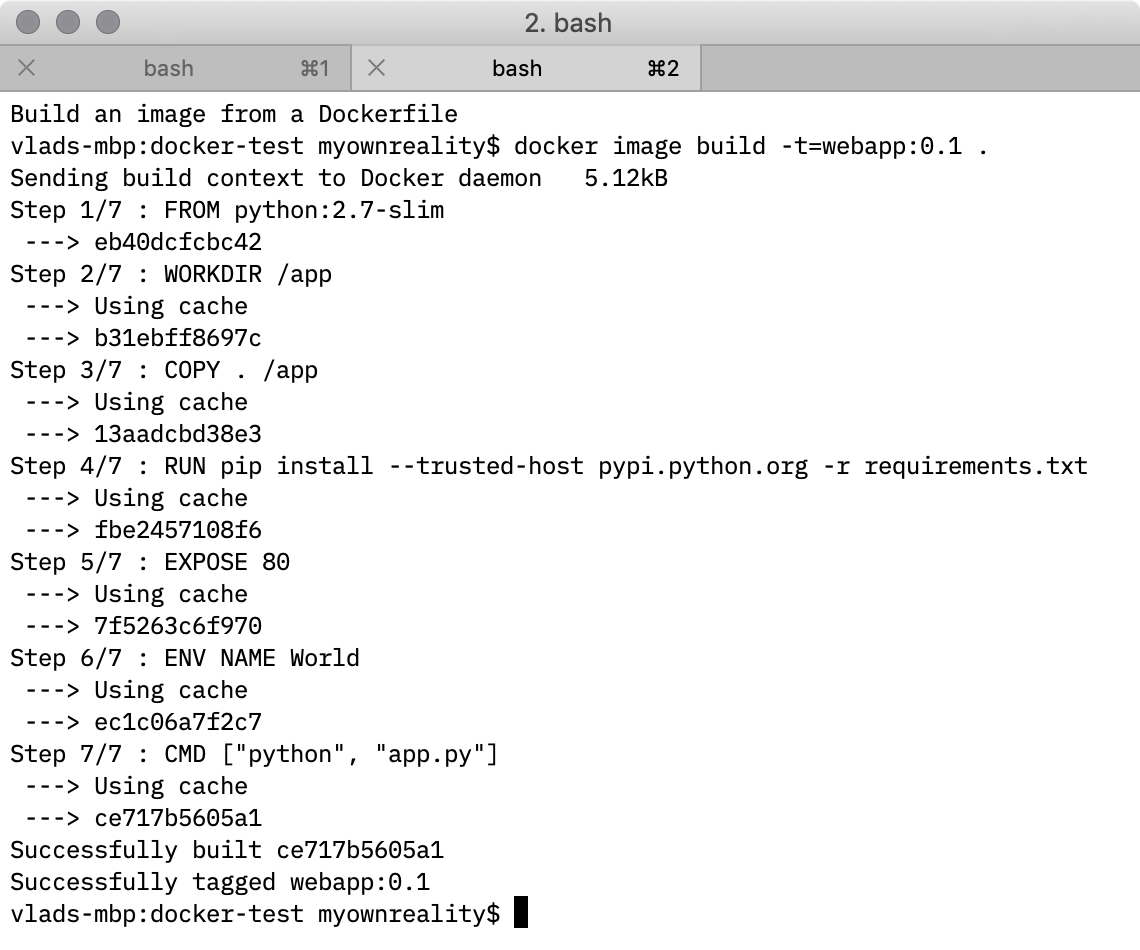
\includegraphics[width=10\gridunitwidth]{./assets/y03s02-syssoft-homework-01-p01.png}
						\caption{Результат побудови образу}
						\label{fig:docker-image-build-res}
					\end{figure}
					
					Переконаємось, що~бажаний образ дійсно створений. Для цього запустимо таку команду:
					\begin{bashterm}
						docker image ls
					\end{bashterm}
					Бачимо, що~створений образ є~у~списку~(рис.~\ref{fig:docker-image-build-res}).

					\begin{figure}[!htbp]
						\centering
						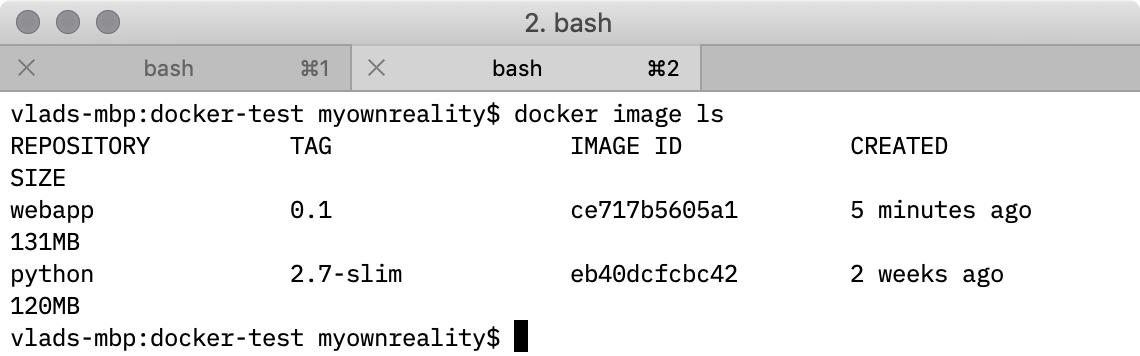
\includegraphics[width=10\gridunitwidth]{./assets/y03s02-syssoft-homework-01-p02.png}
						\caption{Список наявних образів}
						\label{fig:docker-image-ls-res}
					\end{figure}

				\subsubsection{Створення контейнерів з~образів}
					Щоб запустити образ на~виконання, тобто створити контейнер, використовують команду \bashinline|docker run|. Наприклад, запустимо створений контейнер, перенаправивши відкритий порт~80 на~порт~4000 за~допомогою параметра~\bashinline|-p|; також за~допомогою параметра~\bashinline|--rm| вкажемо, що~після завершення роботи контейнер треба видалити. Це~досягається такою командою:
					\begin{bashterm}
						docker run --rm -p 4000:80 webapp:0.1
					\end{bashterm}
					В~результаті контейнер запущений і~працює на~передньому плані~(рис.~\ref{subfig:docker-run-res-term}), а~тому працює і~веб-додаток~(рис.~\ref{subfig:docker-run-res-webapp}).

					\begin{figure}[!htbp]
						\centering
						\begin{subfigure}{\columnwidth}
							\centering
							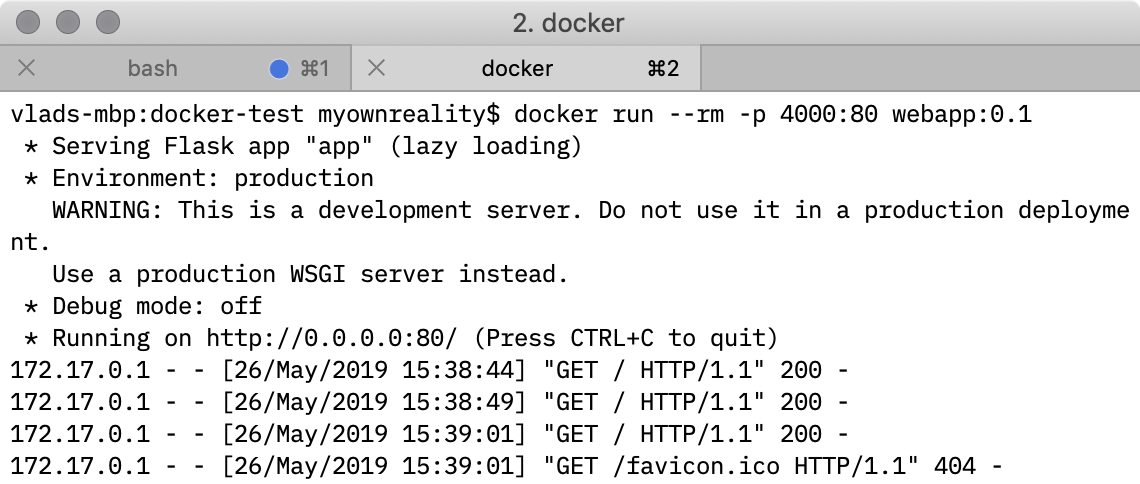
\includegraphics[width=10\gridunitwidth]{./assets/y03s02-syssoft-homework-01-p03a.png}
							\caption{}
							\label{subfig:docker-run-res-term}
						\end{subfigure}
						\begin{subfigure}{\columnwidth}
							\centering
							
\includegraphics[width=10\gridunitwidth]{./assets/y03s02-syssoft-homework-01-p03b.png}
							\caption{}
							\label{subfig:docker-run-res-webapp}
						\end{subfigure}
						\caption{Результат створення і~запуску контейнера: \subref{subfig:docker-run-res-term}~— вікно терміналу, \subref{subfig:docker-run-res-webapp}~— веб-додаток у~браузері}
						\label{fig:docker-run-res}
					\end{figure}

					Найчастіше контейнери запускають у~фоновому режимі, тобто на~задньому плані. У~такому випадку контейнер не~займає термінал, а~виконується у~фоновому процесі. Тим не~менш, він доступний для управління і~відстеження за~допомогою спеціальних команд.
					
					Отже, запустимо контейнер так само, як~і~у~попередній раз, але тепер у~фоновому режимі за~допомогою параметра~\bashinline|-d|. Для цього спочатку перейдемо у~активне вікно емулятора термінала і~завершимо виконання контейнера, який працює на~передньому плані, натиснувши комбінацію клавіш \textenglish{Ctrl + C}, а~потім запустимо контейнер за~допомогою відповідної команди:
					\begin{bashterm}
						docker run -d --rm -p 4000:80 webapp:0.1
					\end{bashterm}
					В~результаті побачимо, що~у~вікно емулятора термінала був виведений ідентифікатор запущеного контейнера. Перевіримо, які команди зараз запущені. Для цього виконаємо таку команду:
					\begin{bashterm}
						docker ps
					\end{bashterm}
					Бачимо, що~контейнер запущений на~виконання і~успішно працює~(рис.~\ref{subfig:docker-run-d-res-term}). Отже, працює і~веб-додаток~(рис.~\ref{subfig:docker-run-d-res-webapp}).

					\begin{figure}[!htbp]
						\centering
						\begin{subfigure}{\columnwidth}
							\centering
							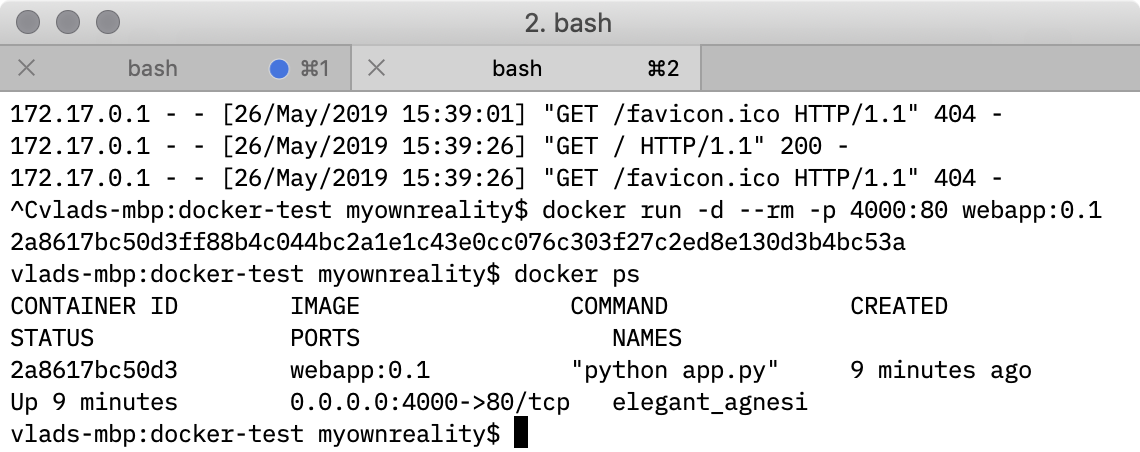
\includegraphics[width=10\gridunitwidth]{./assets/y03s02-syssoft-homework-01-p04a.png}
							\caption{}
							\label{subfig:docker-run-d-res-term}
						\end{subfigure}
						\begin{subfigure}{\columnwidth}
							\centering
							
\includegraphics[width=10\gridunitwidth]{./assets/y03s02-syssoft-homework-01-p04b.png}
							\caption{}
							\label{subfig:docker-run-d-res-webapp}
						\end{subfigure}
						\caption{Результат запуску контейнера у~фоновому режимі: \subref{subfig:docker-run-d-res-term}~— вікно терміналу, \subref{subfig:docker-run-d-res-webapp}~— веб-додаток у~браузері}
						\label{fig:docker-run-d-res}
					\end{figure}

					Тепер зупинимо працюючий контейнер. Для цього використовується команда~\bashinline|docker stop|. Як~видно з~вікна терміналу~(рис.~\ref{subfig:docker-run-d-res-term}), запущений контейнер має ідентифікатор~\bashinline|2a8617bc50d3|. Щоб зупинити цей контейнер, виконаємо таку команду:
					\begin{bashterm}
						docker stop 2a8617bc50d3
					\end{bashterm}
					В~результаті контейнер був зупинений~(рис.\ref{fig:docker-stop-res}).

					\begin{figure}[!htbp]
						\centering
						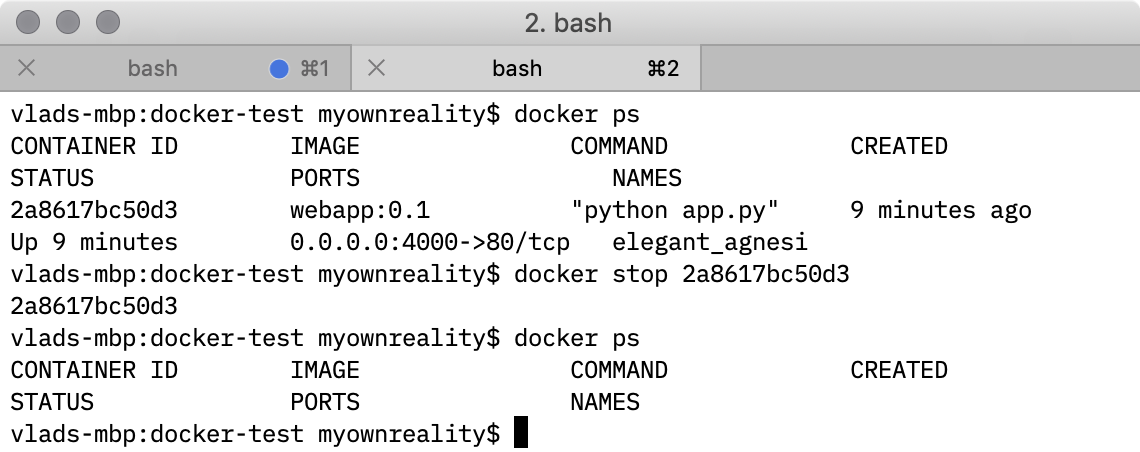
\includegraphics[width=10\gridunitwidth]{./assets/y03s02-syssoft-homework-01-p05.png}
						\caption{Зупинка контейнера, який працює у~фоновому режимі}
						\label{fig:docker-stop-res}
					\end{figure}

			\subsection{Сервіси}
				Сервіси~— це~різні частини розподіленого програмного забезпечення. Наприклад, у~програмного забезпеченні, яке ми~розглядаємо для прикладу, є~два сервіси: веб-додаток і~база даних. Взагалі, сервіси можна вважати «контейнерами у~роботі»~(\transeng{containers in production}), тому що~сервіс виконує лише один образ, але описує параметри, як~цей образ повинен виконуватись: які порти використовувати, які мережі використовувати, при яких умовах перезавантажуватись тощо.

				Використання сервісів дозволяє зручно визначати багатоконтейнерні інстанції для прикладних програм. Оскільки в~програми, яка розглядається для прикладу, передбачено два сервіси, розглянемо її.

				\subsubsection{Опис сервісів}
					Зручну роботу з~сервісами забезпечує утиліта~\textenglish{Docker Compose}, яка дозволяє створювати і~управляти сервісами. При роботі з~\textenglish{Docker Compose}, сервіси описують за~допомогою спеціальних файлів~\filename{\textenglish{docker-compose.yml}}. Опишемо сервіси для нашої програми.

					Як~було сказано раніше, програма складається з~двох сервісів: веб-додатку і~бази даних. Щоб це~описати, у~директорії проекту створюємо відповідний файл~\filename{\textenglish{docker-compose.yml}}~(лістинг~\ref{lst:docker-compose-01}).

					\begin{listingdockercompose}{Файл~\filename{\textenglish{docker-compose.yml}} для опису сервісів програми}{lst:docker-compose-01}
            # Використовувати Docker Compose версії 3
            version: "3"
            # Опис сервісів
            services:
              # Сервіс "webapp"
              webapp:
                # Використати образ "webapp:0.1"
                image: "webapp"
                # Перенаправити порти
                ports:
                  # На~порт хоста 4000 перенаправити порт контейнера 80
                  - "4000:80"
              # Сервіс "database"
              database:
                # Використати образ "redis"
                image: "redis"
                volumes:
                  # Прив'язати том "dbvolume" на~хості до~директорії "/data"
                  # всередині контейнера
                  - "dbvolume:/data"

            # Опис томів
            volumes:
              # Оголосити "dbvolume", щоб дані сервісу "database" зберігались
              # навіть після зупинки контейнера. Дані будуть збережені доти,
              # доки том "dbvolume" не~буде видалений
              dbvolume:
					\end{listingdockercompose}
					Описавши всі сервіси, необхідні для роботи програми, можна переходити до~їх~запуску.

				\subsubsection{Запуск і~управління сервісами}
					Тепер запустимо всі описані сервіси нашої програми за~допомогою утиліти \textenglish{Docker Compose}. Для цього виконаємо таку команду:
					\begin{bashterm}
						docker-compose up
					\end{bashterm}
					В~результаті бачимо, що~запускаються два сервіси: база даних~\progname{database} і~веб-додаток~\progname{webapp}~(рис.~\ref{subfig:docker-compose-up-res-term}). Оскільки база даних запущена і~працює, тепер лічильник справний~(рис.~\ref{subfig:docker-compose-up-res-webapp}). Якщо ж~сервіси треба запустити у~фоновому режимі, аналогічно до~контейнерів, необхідно виконати вищезазначену команду з~параметром~\bashinline|-d|.

					\begin{figure}[!htbp]
						\centering
						\begin{subfigure}{\columnwidth}
							\centering
							
\includegraphics[width=10\gridunitwidth]{./assets/y03s02-syssoft-homework-01-p06a.png}
							\caption{}
							\label{subfig:docker-compose-up-res-term}
						\end{subfigure}
						\begin{subfigure}{\columnwidth}
							\centering
							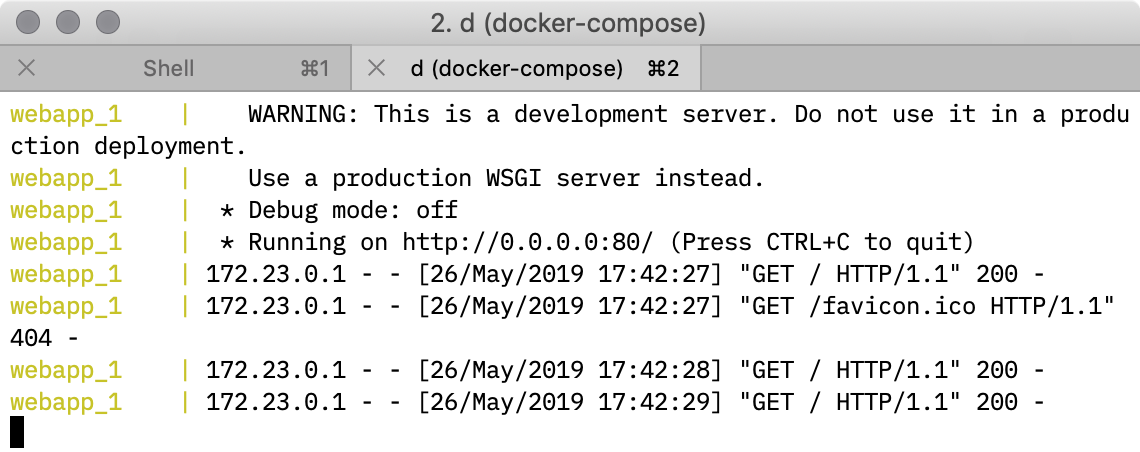
\includegraphics[width=10\gridunitwidth]{./assets/y03s02-syssoft-homework-01-p06b.png}
							\caption{}
							\label{subfig:docker-compose-up-res-webapp}
						\end{subfigure}
						\caption{Результат запуску мультисервісної програми: \subref{subfig:docker-run-d-res-term}~— вікно терміналу, \subref{subfig:docker-run-d-res-webapp}~— веб-додаток у~браузері}
						\label{fig:docker-compose-up-res}
					\end{figure}

					Зупинимо запущені сервіси. Оскільки вони працюють на~передньому плані, щоб їх~зупинити достатньо натиснути комбінацію клавіш~\textenglish{Ctrl + C}. Після цього всі сервіси, запущені за~описаним файлом~\filename{\textenglish{docker-compose.yml}} будуть зупинені. Однак, це~не~означає, що~була видалена вся інфраструктура, створена \textenglish{Docker Compose}: ще~залишились створена мережа, в~якій знаходяться описані сервіси, а~також том~«\textenglish{dbvolume}».

					Щоб видалити створену інфраструктуру, тобто повністю зупинити сервіси і~почистити результати їх~виконання, треба виконати таку команду:
					\begin{bashterm}
						docker-compose down
					\end{bashterm}
					В~результаті її~виконання будуть видалені усі мережі, томи та~інші артефакти, описані у~файлі~\filename{\textenglish{docker-compose.yml}}.

			\section{Висновок}
				Виконуючи дане домашнє завдання, ми~ознайомились і~описали платформу~\textenglish{Docker}. Ця~платформа призначена для контейнеризації прикладних програм, що~дозволяє зручно розповсюджувати програми, не~переймаючись, що~вони не~запустяться на~інших комп'ютерах.

				Крім того, платформа~\textenglish{Docker} дозволяє ізолювати складові програмного продукту, не~заважаючи обміну даних між ними, завдяки сервісам і~спеціальним утилітам на~кшталт~\textenglish{Docker Compose}, стеків і~роїв. У~рамках даного домашнього завдання ми~розглянули розгортання багатосервісного програмного продукту за~допомогою утиліти~\textenglish{Docker Compose}, яка дозволила зручно обмінюватись даними між описаними сервісами як~за~допомогою мережі, так і~за~допомогою файлової системи.

				Загалом, завдяки відтворюваності об'єктів, які створюються інструментами платформи~\textenglish{Docker}, а~також зручному управлінню за~допомогою утиліт, які вона надає, ця~платформа значно спрощує процес розробки, тестування і~доставки розроблених програм кінцевим користувачам.
\end{document}

